% !TEX encoding = UTF-8 Unicode
% !TEX root = thesis-ex.tex
This discussion is based on the measurement described in \cite{PhysRevC.98.024908}.
While measurements like \RAA \cite{} and asymmetry \cite{} describe how much energy is lost by the jet, fragmentation measurements describe the momentum distribution of particles associated to the jet.
These can be described as:

\begin{align}
\Dz = \frac{1}{\Njet} \frac{d\nch}{dz} \\
\Dpt = \frac{1}{\Njet} \frac{d\nch}{d\pt}
\end{align}
where $z = \pt \cos(\Delta R / \ptjet)$ and gives the charged-particle longitudinal momentum fraction relative to the jet.
Modifications to the fragmentation functions in \pbpb\ collisions can be evaluated by constructing the ratios: 

\begin{align}
\Rdz = \frac{\Dz_{\pbpb}}{\Dz_{\pp}} \\
\Rdpt = \frac{\Dpt_{\pbpb}}{\Dpt_{\pp}} 
\end{align}
This measurement is corrected for detector effects and unfolded to the particle level.
This allows for comparisons to other measurements and theoretical models.
The \Dz\ and \Dpt\ distributions are shown in Figure~\ref{fig:jetff_dz} and Figure~\ref{fig:jetff_dpt} 

\begin{figure}[htbp]
\begin{center}
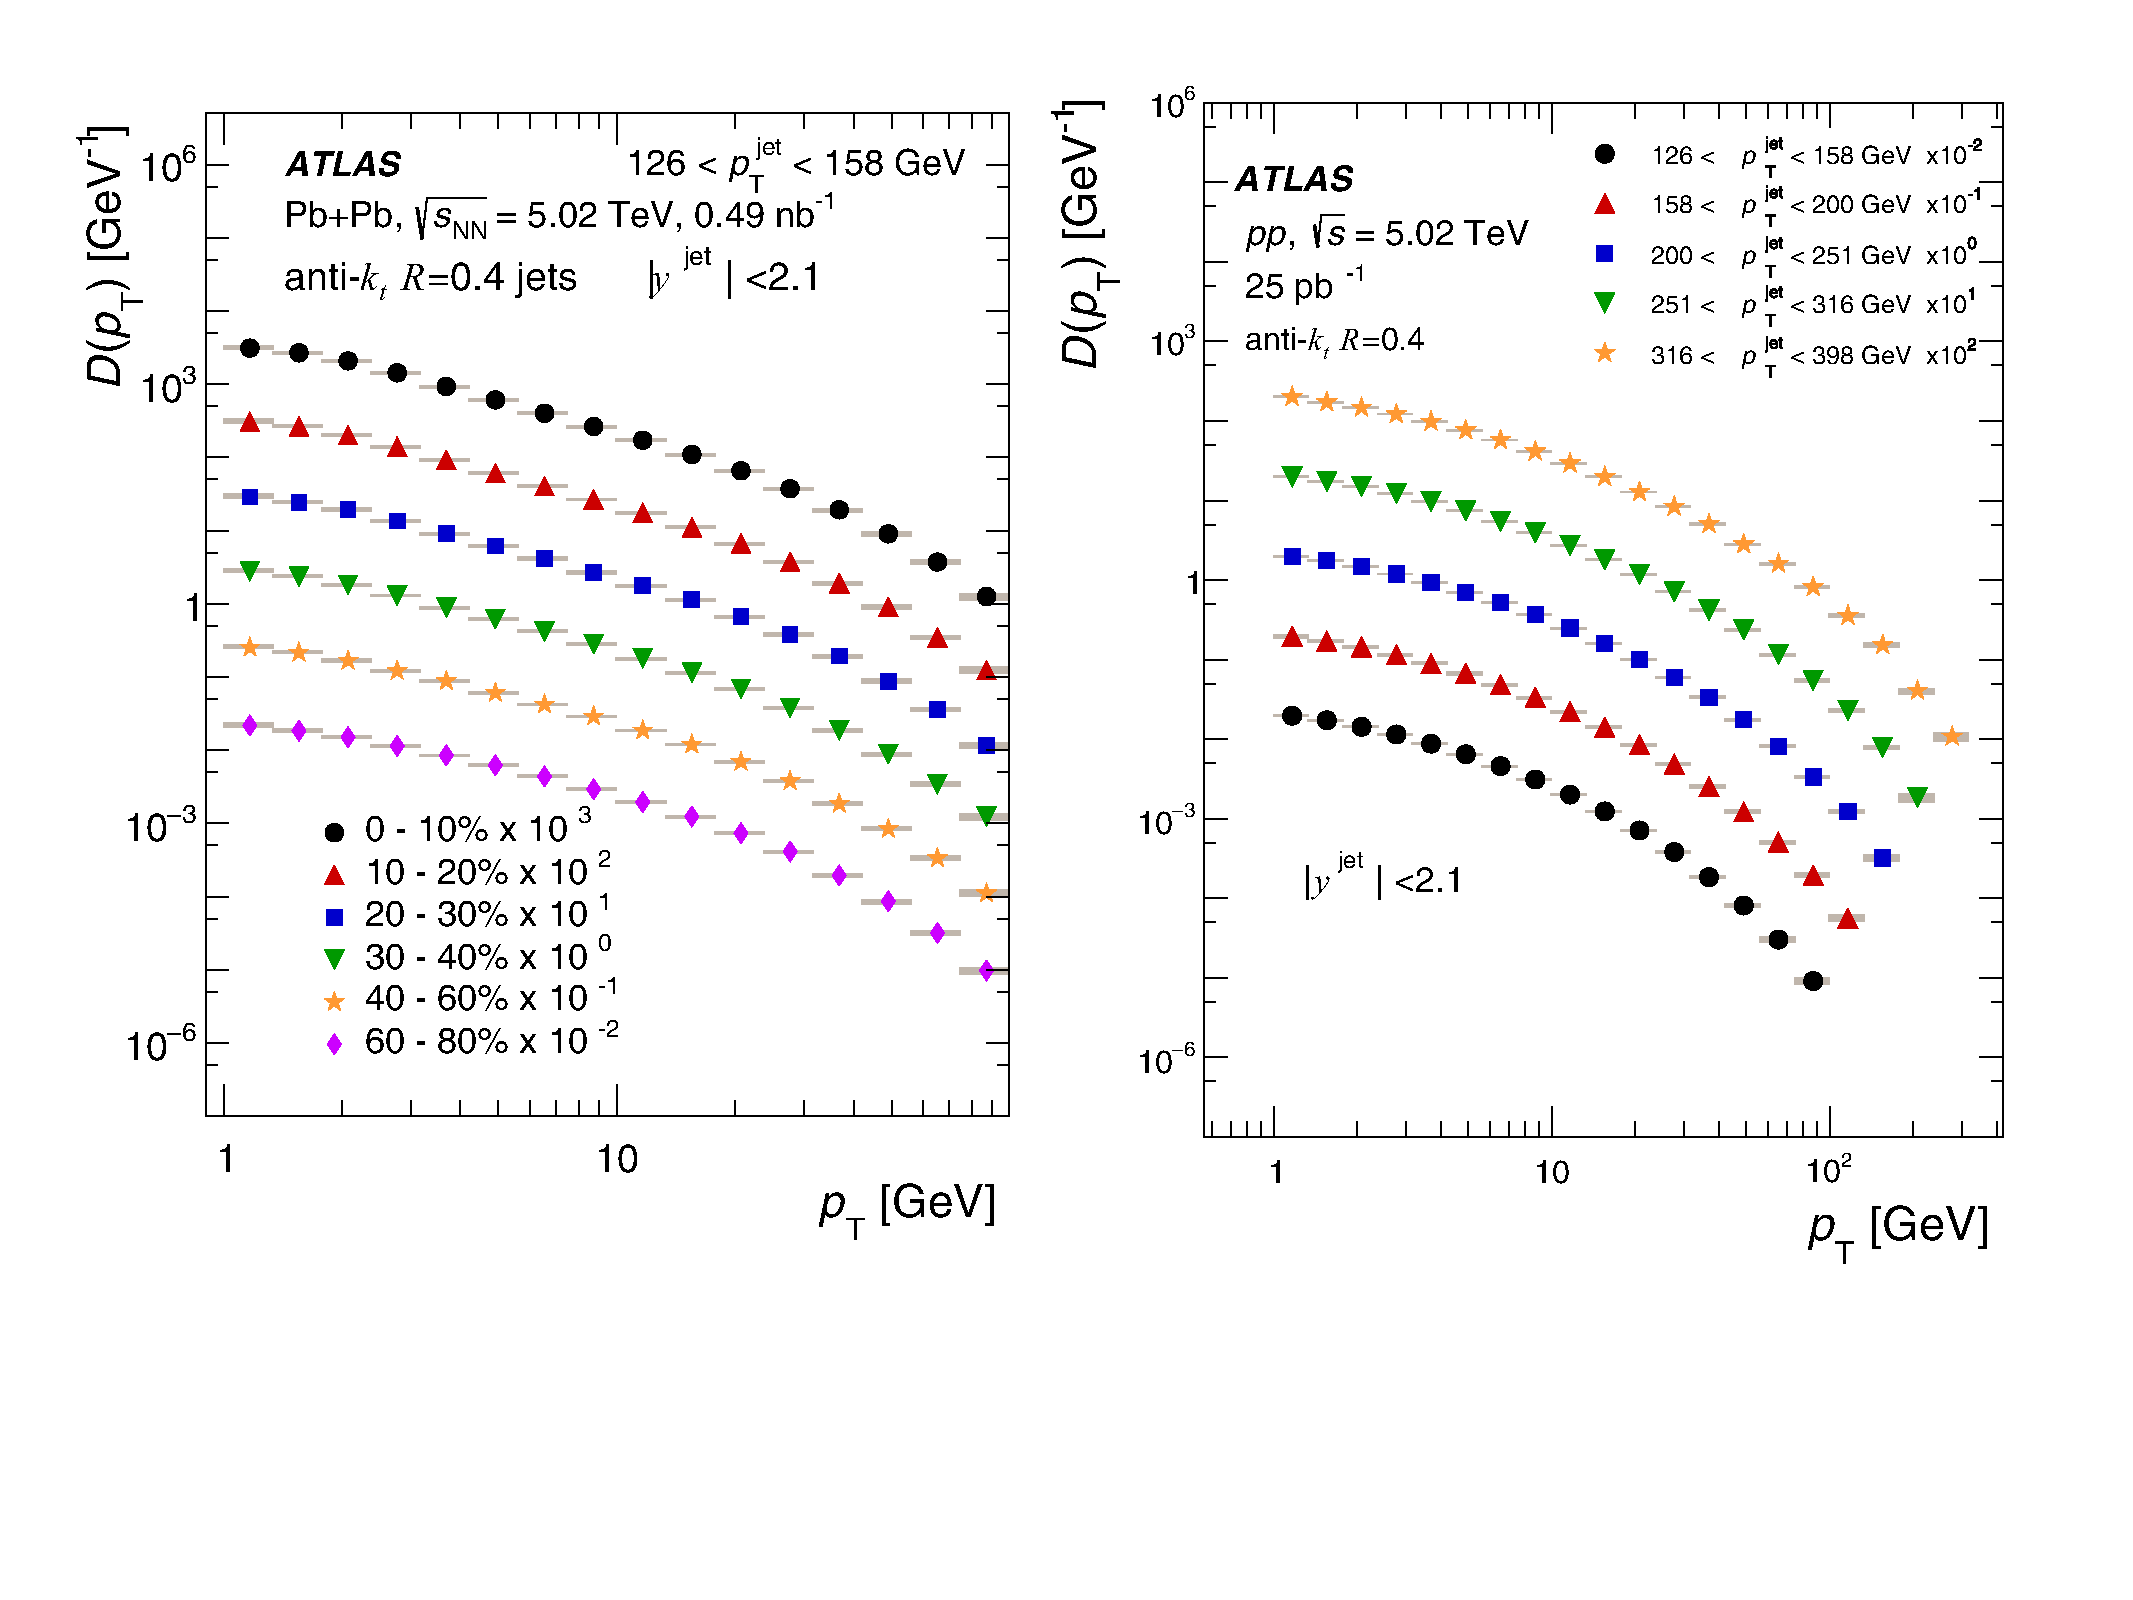
\includegraphics[width=0.55\textwidth]{figures/jetMeasurements/jetff_dpt}
\caption{(Left) The \Dpt\ distributions in \pp\ as a function of charged-particle \pt\ for different \ptjet\ selections and for jet rapidity $|y| < 2.1$.
(Right) The \Dpt\ distributions in \pbpb\ as a function of charged-particle \pt\ for different centrality selections and for jet rapidity $|y| < 2.1$.
The error bars represent statistical uncertainties while the shaded boxes represent systematic uncertainties.
Figure taken from \cite{PhysRevC.98.024908}.}
\label{fig:jetff_dpt}
\end{center}
\end{figure}


\begin{figure}[htbp]
\begin{center}
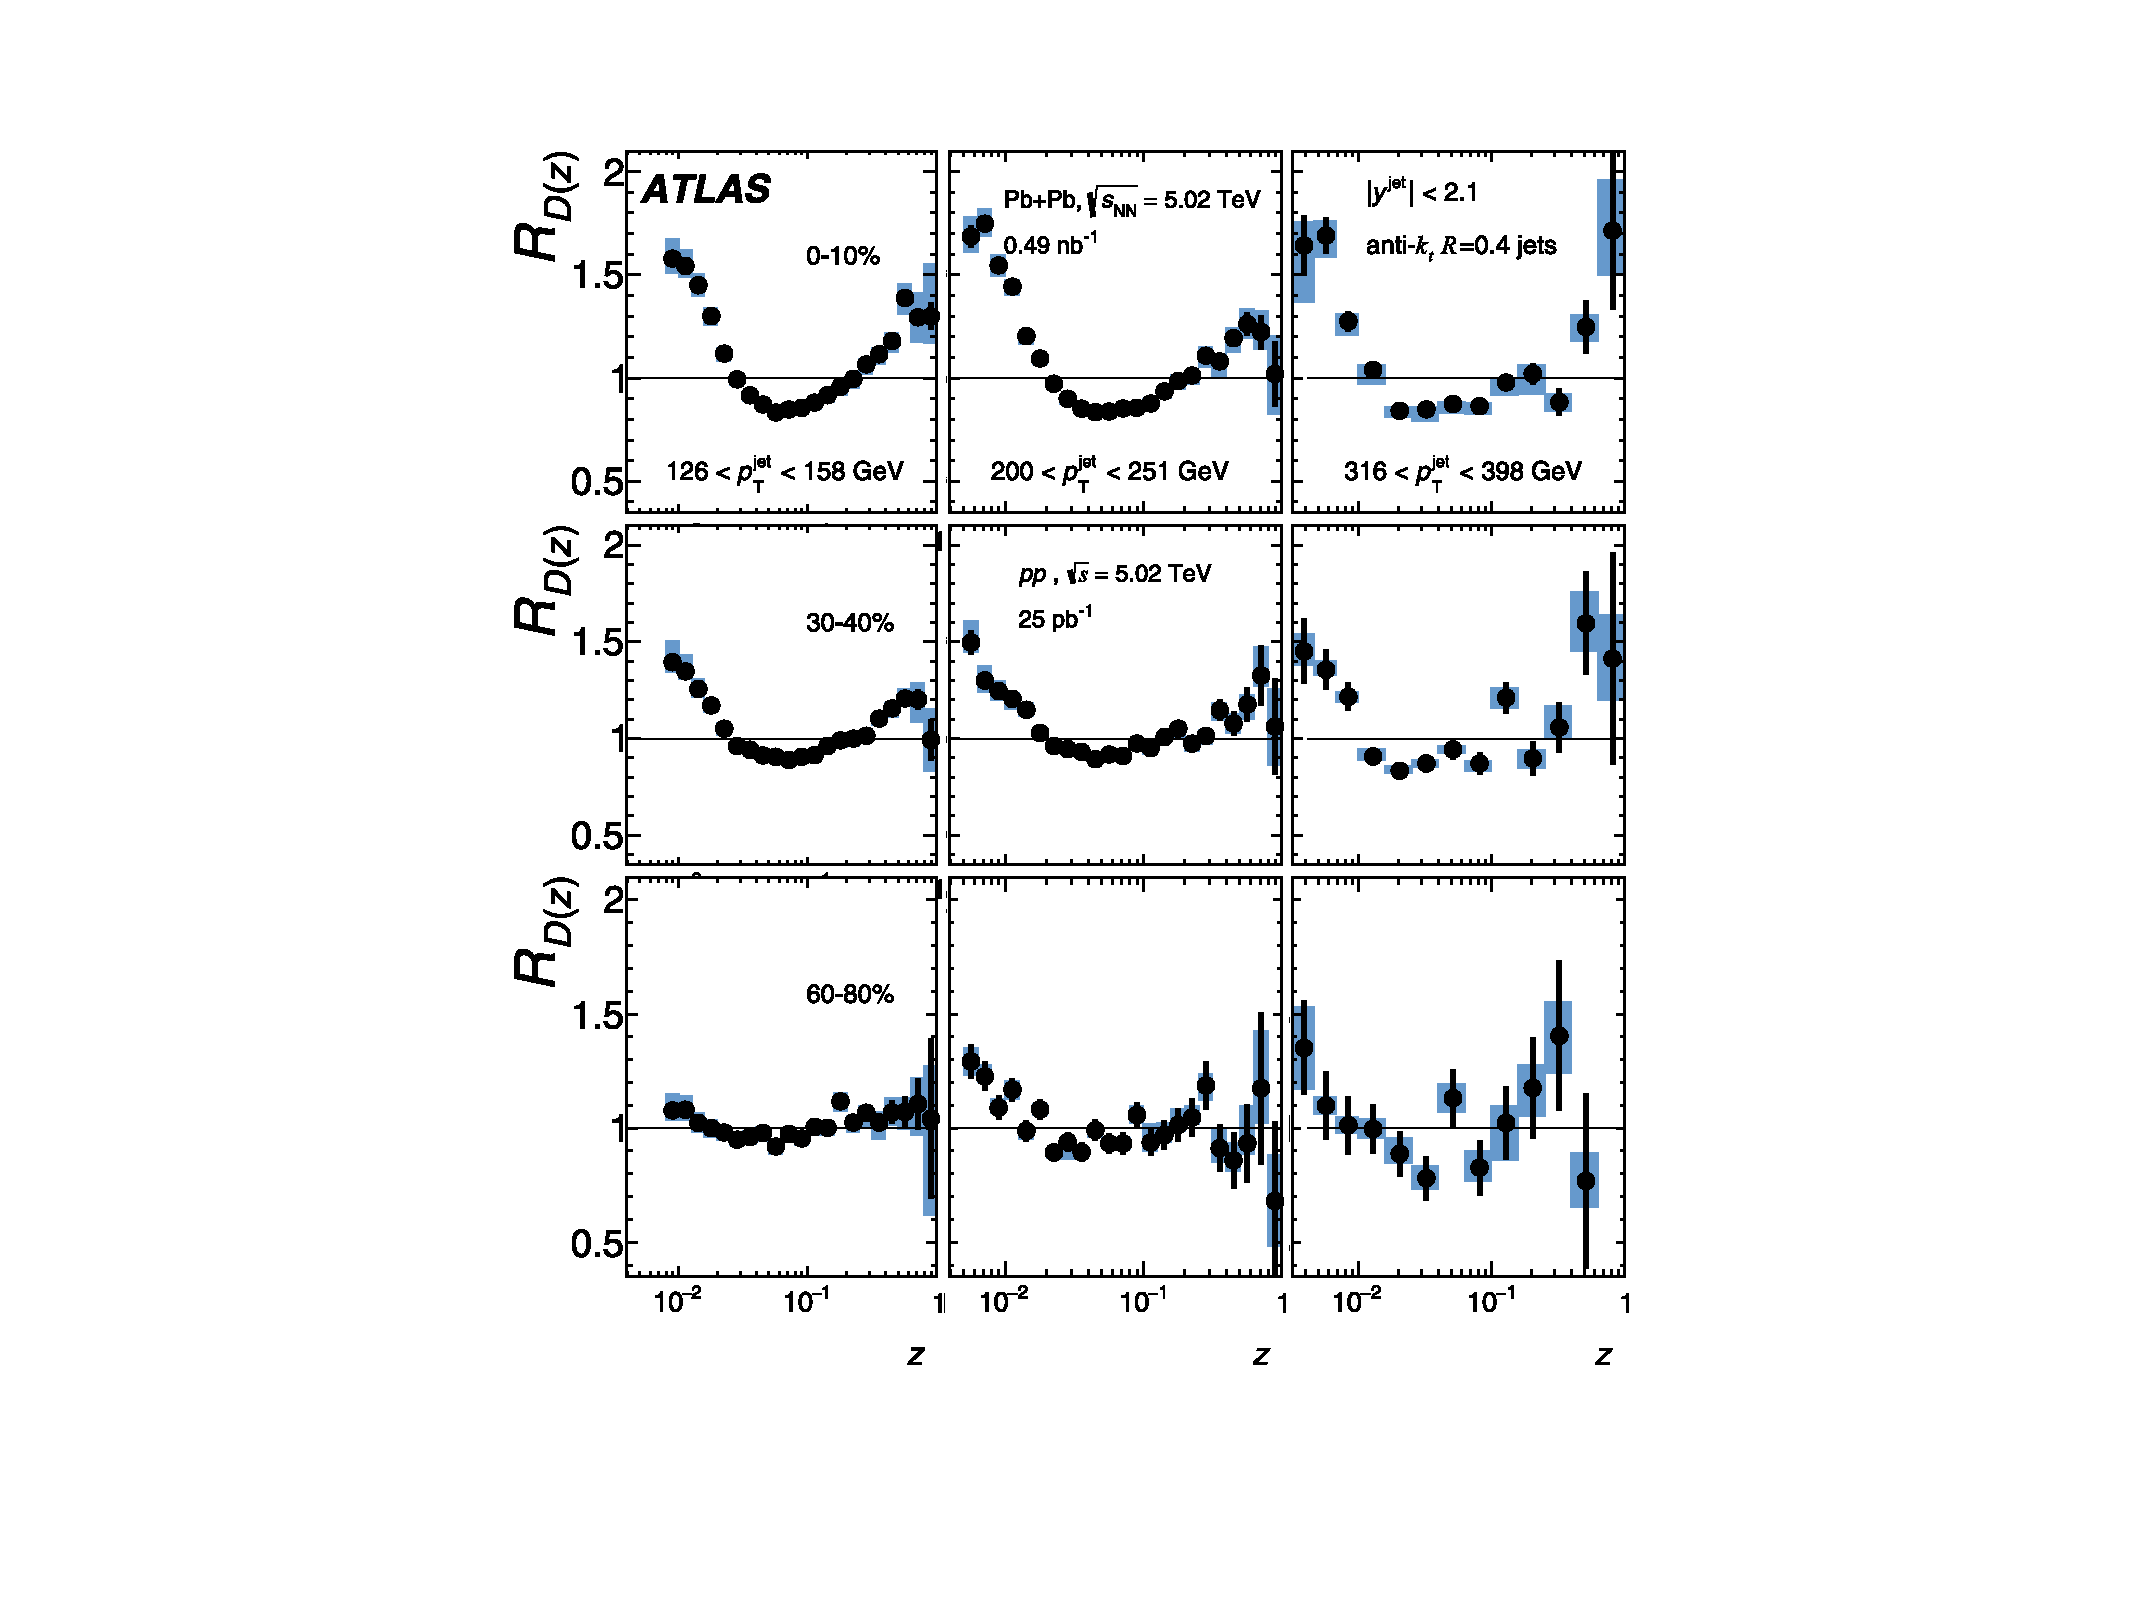
\includegraphics[width=0.55\textwidth]{figures/jetMeasurements/jetff_rdz}
\caption{The modifications to the \Dz\ distributions in \pbpb\ compared to \pp\ as a function of charged-particle $z$ for different \ptjet\ selections (left to right) and different centrality selections (top to bottom) for jet rapidity $|y| < 0.3$.
The error bars represent statistical uncertainties while the shaded boxes represent systematic uncertainties.
Figure taken from \cite{PhysRevC.98.024908}.}
\label{fig:jetff_rdz}
\end{center}
\end{figure}

The modifications to the \Dz\ distributions are shown in Figure~\ref{fig:jetff_rdz}.
It can be seen that there is an excess of particles with low $z$ and high $z$.
These are particles that carry either a small or a large fraction of energy of the jet \pt.
There is an associated depletion for particles with intermediate $z$.
These modifications become smaller for more peripheral collisions.
The \ptjet\ dependence of the \Rdz\ and \Rdpt\ distributions can be seen in Figure~\ref{fig:jetff_jetpt_dep}.
This dependence can give insight into the modification of the fragmentation functions, with any scaling with $z$ indicating a change in the fragmentation pattern, while a scaling with \pt\ reflecting an effect from the medium itself.
The low momentum excess in the \Rdpt\ distributions seen in Figure~\ref{fig:jetff_jetpt_dep} can be further studied by integrating over that region.
Then the extra number of particles in \pbpb\ compared to \pp\ is given by:

\begin{align}
\Nch = \int^{\pt_{\mathrm{max}}}_{\pt_{\mathrm{min}}} \left( \Dpt_{\pbpb} - \Dpt_{\pp} \right) d\pt
\end{align}
where $\pt_{\mathrm{min}} = 1$ GeV and $\pt_{\mathrm{max}} = 4.2$ GeV.
The \Nch\ distributions can be seen in Figure~\ref{fig:jetff_nch}.
It can be clearly seen that the size of the excess increases as a function of \ptjet, growing from about 1.5 to 2.5 extra particles in the most central \pbpb\ collisions.
This excess is even seen in the peripheral \pbpb\ collisions, though it is a lot smaller and ranges from 0.2 to 0.5 extra particles.




\begin{figure}[htbp]
\begin{center}
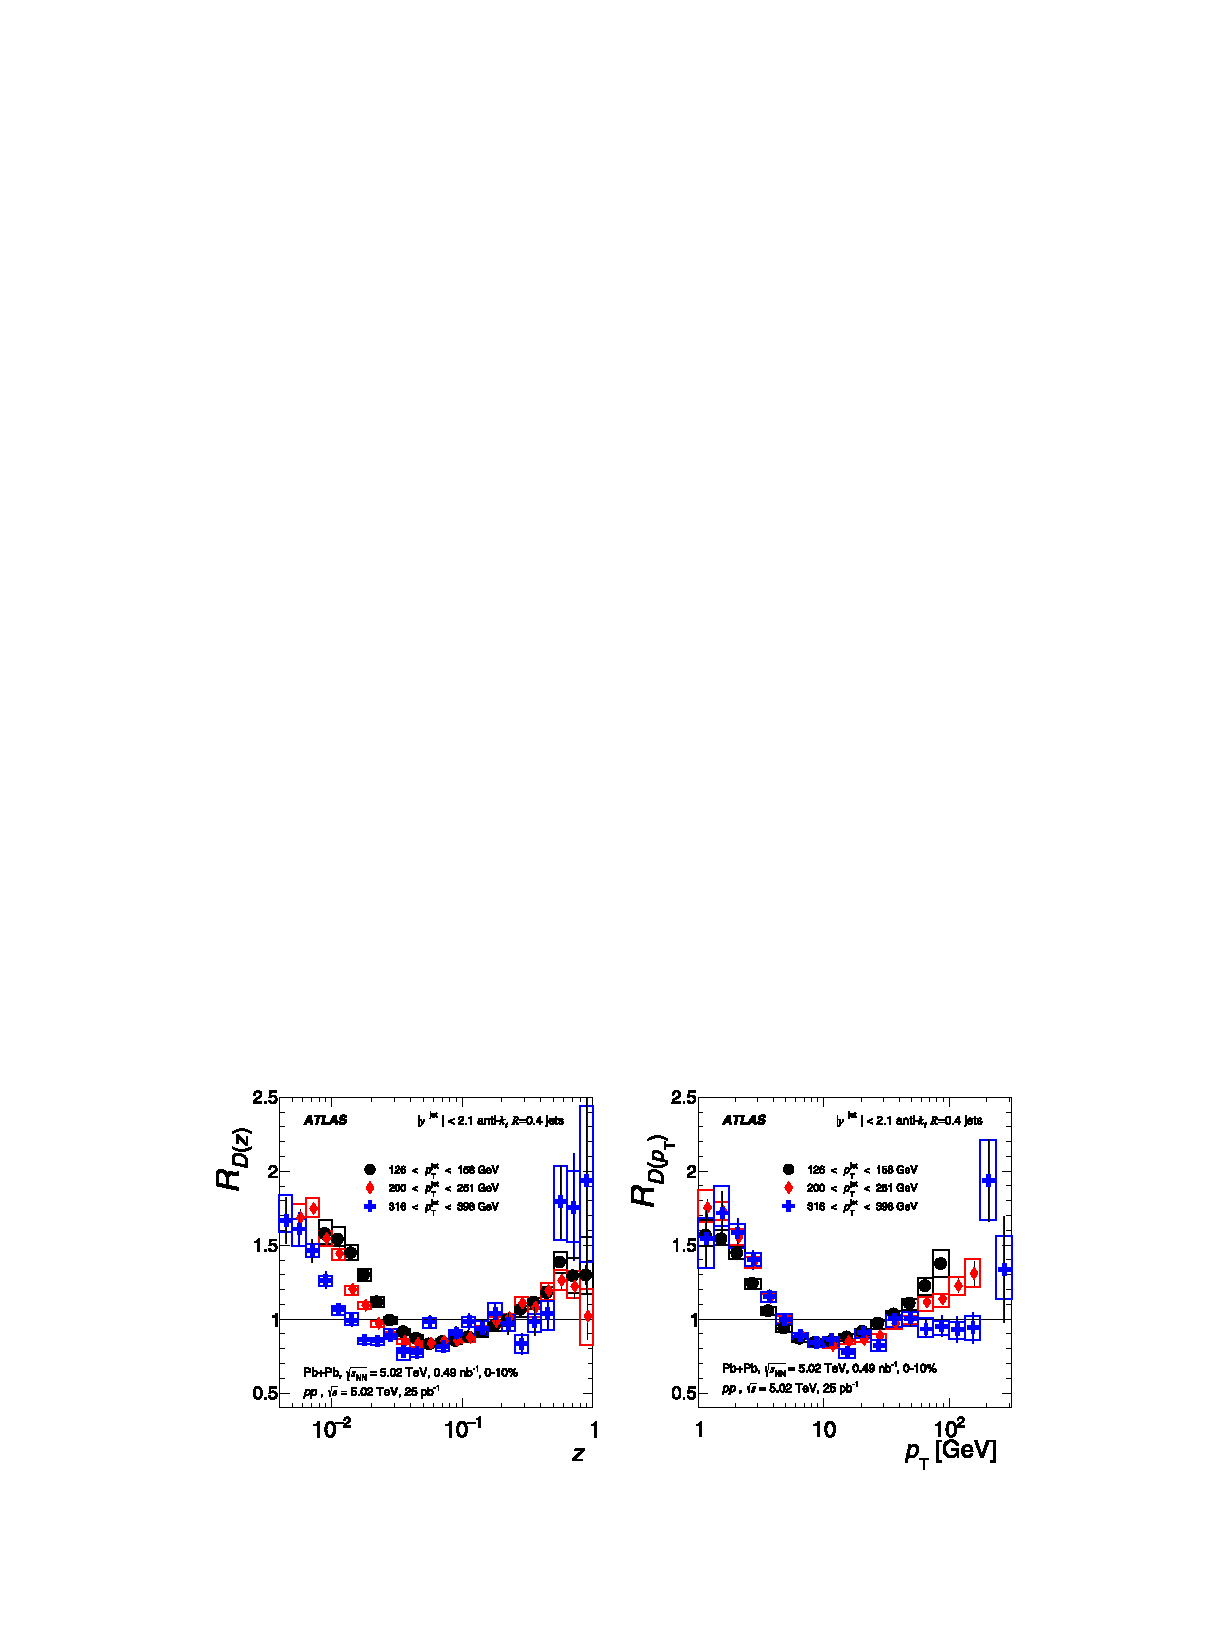
\includegraphics[width=0.75\textwidth]{figures/jetMeasurements/jetff_jetpt_dep}
\caption{The \ptjet\ dependence of the \Rdz\ (left) and \Rdpt\ (right) distributions in 0--10\% central \pbpb\ compared to \pp\ collisions.
The error bars represent statistical uncertainties while the shaded boxes represent systematic uncertainties.
Figure taken from \cite{PhysRevC.98.024908}.}
\label{fig:jetff_jetpt_dep}
\end{center}
\end{figure}


\begin{figure}[htbp]
\begin{center}
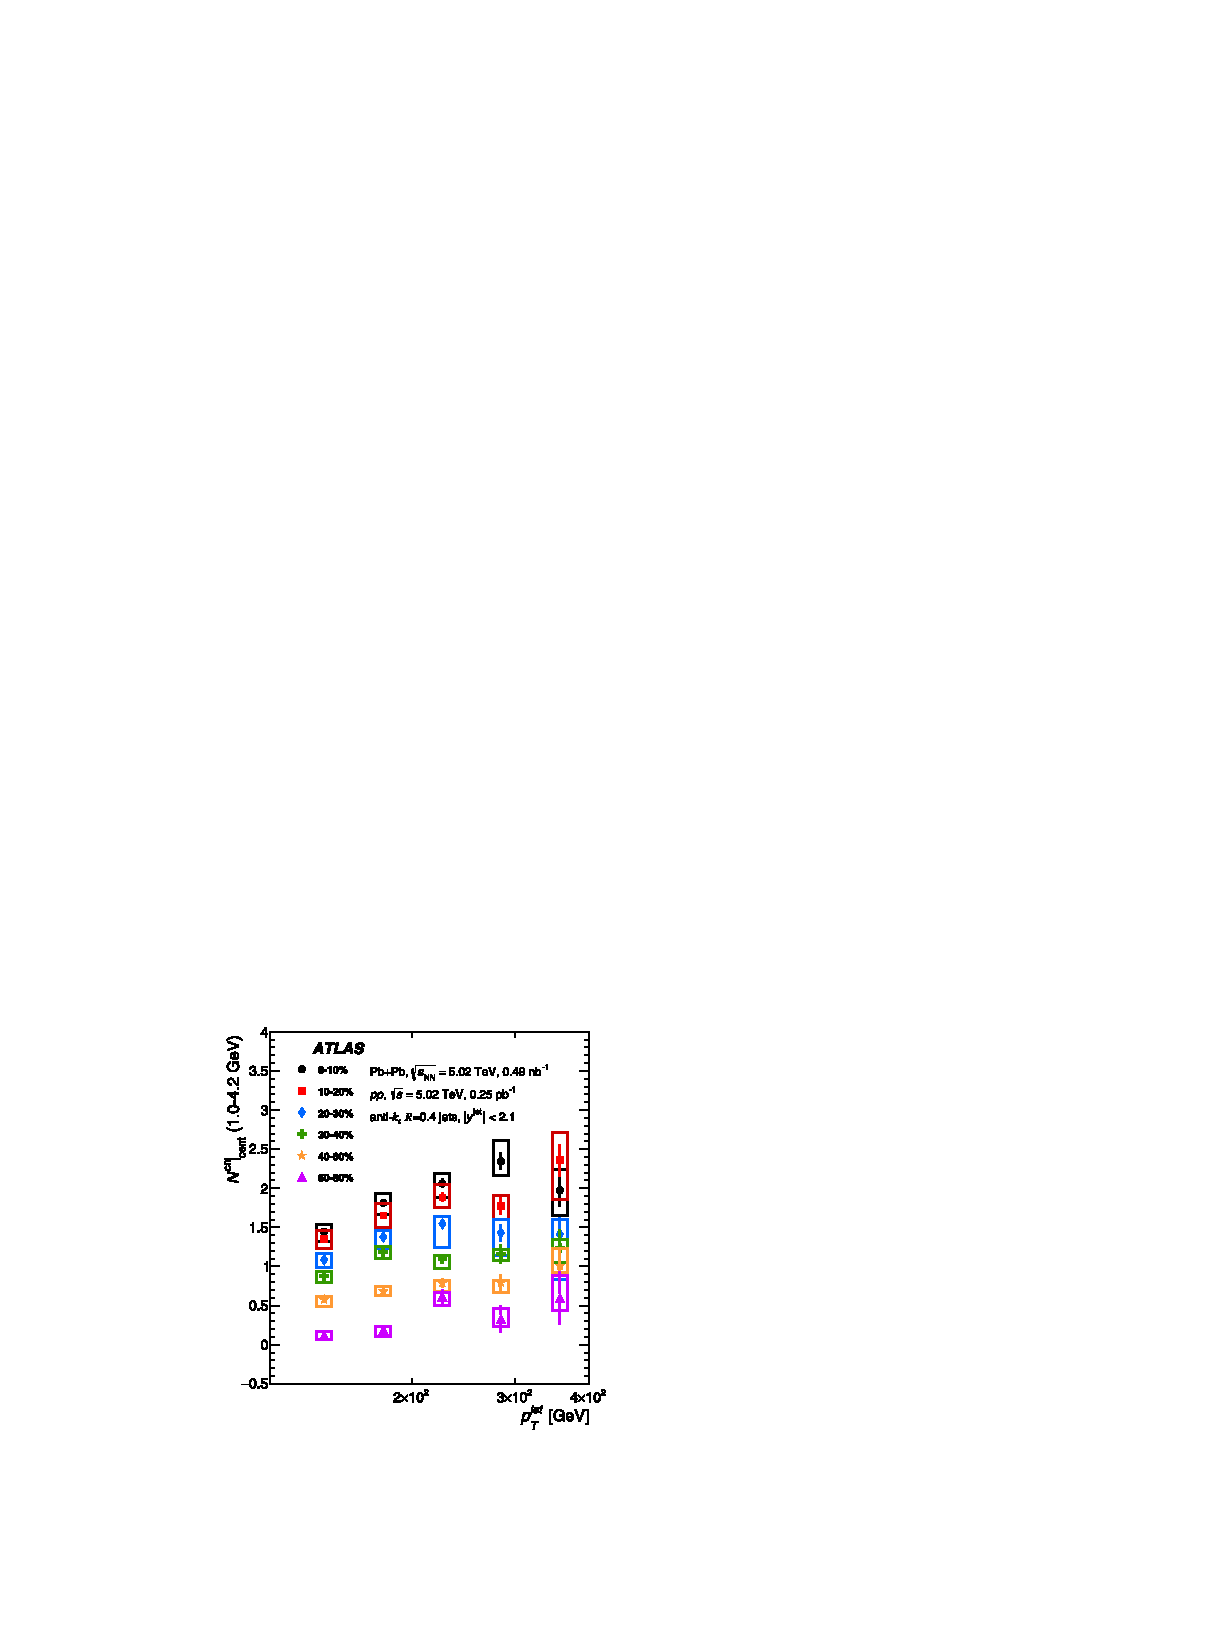
\includegraphics[width=0.35\textwidth]{figures/jetMeasurements/jetff_nch}
\caption{The number of extra particles that carry $1<\pt<4$ GeV  in \pbpb\ compared to \pp.
The different colors represent different centrality selections.
The error bars represent statistical uncertainties while the shaded boxes represent systematic uncertainties.
Figure taken from \cite{PhysRevC.98.024908}.}
\label{fig:jetff_nch}
\end{center}
\end{figure}

The modifications to the \Dz\ distributions have also been compared to a variety of models, including the Effective Quenching model \cite{Spousta:2015fca}, the Soft Collinear Effective Theory \cite{Chien:2015vja, Kang:2017frl}, and the Hybrid Model \cite{Casalderrey-Solana:2014bpa}.
These comparisons are shown in Figure~\ref{fig:jetff_rdz_theory}.
It can be seen that...


\begin{figure}[htbp]
\begin{center}
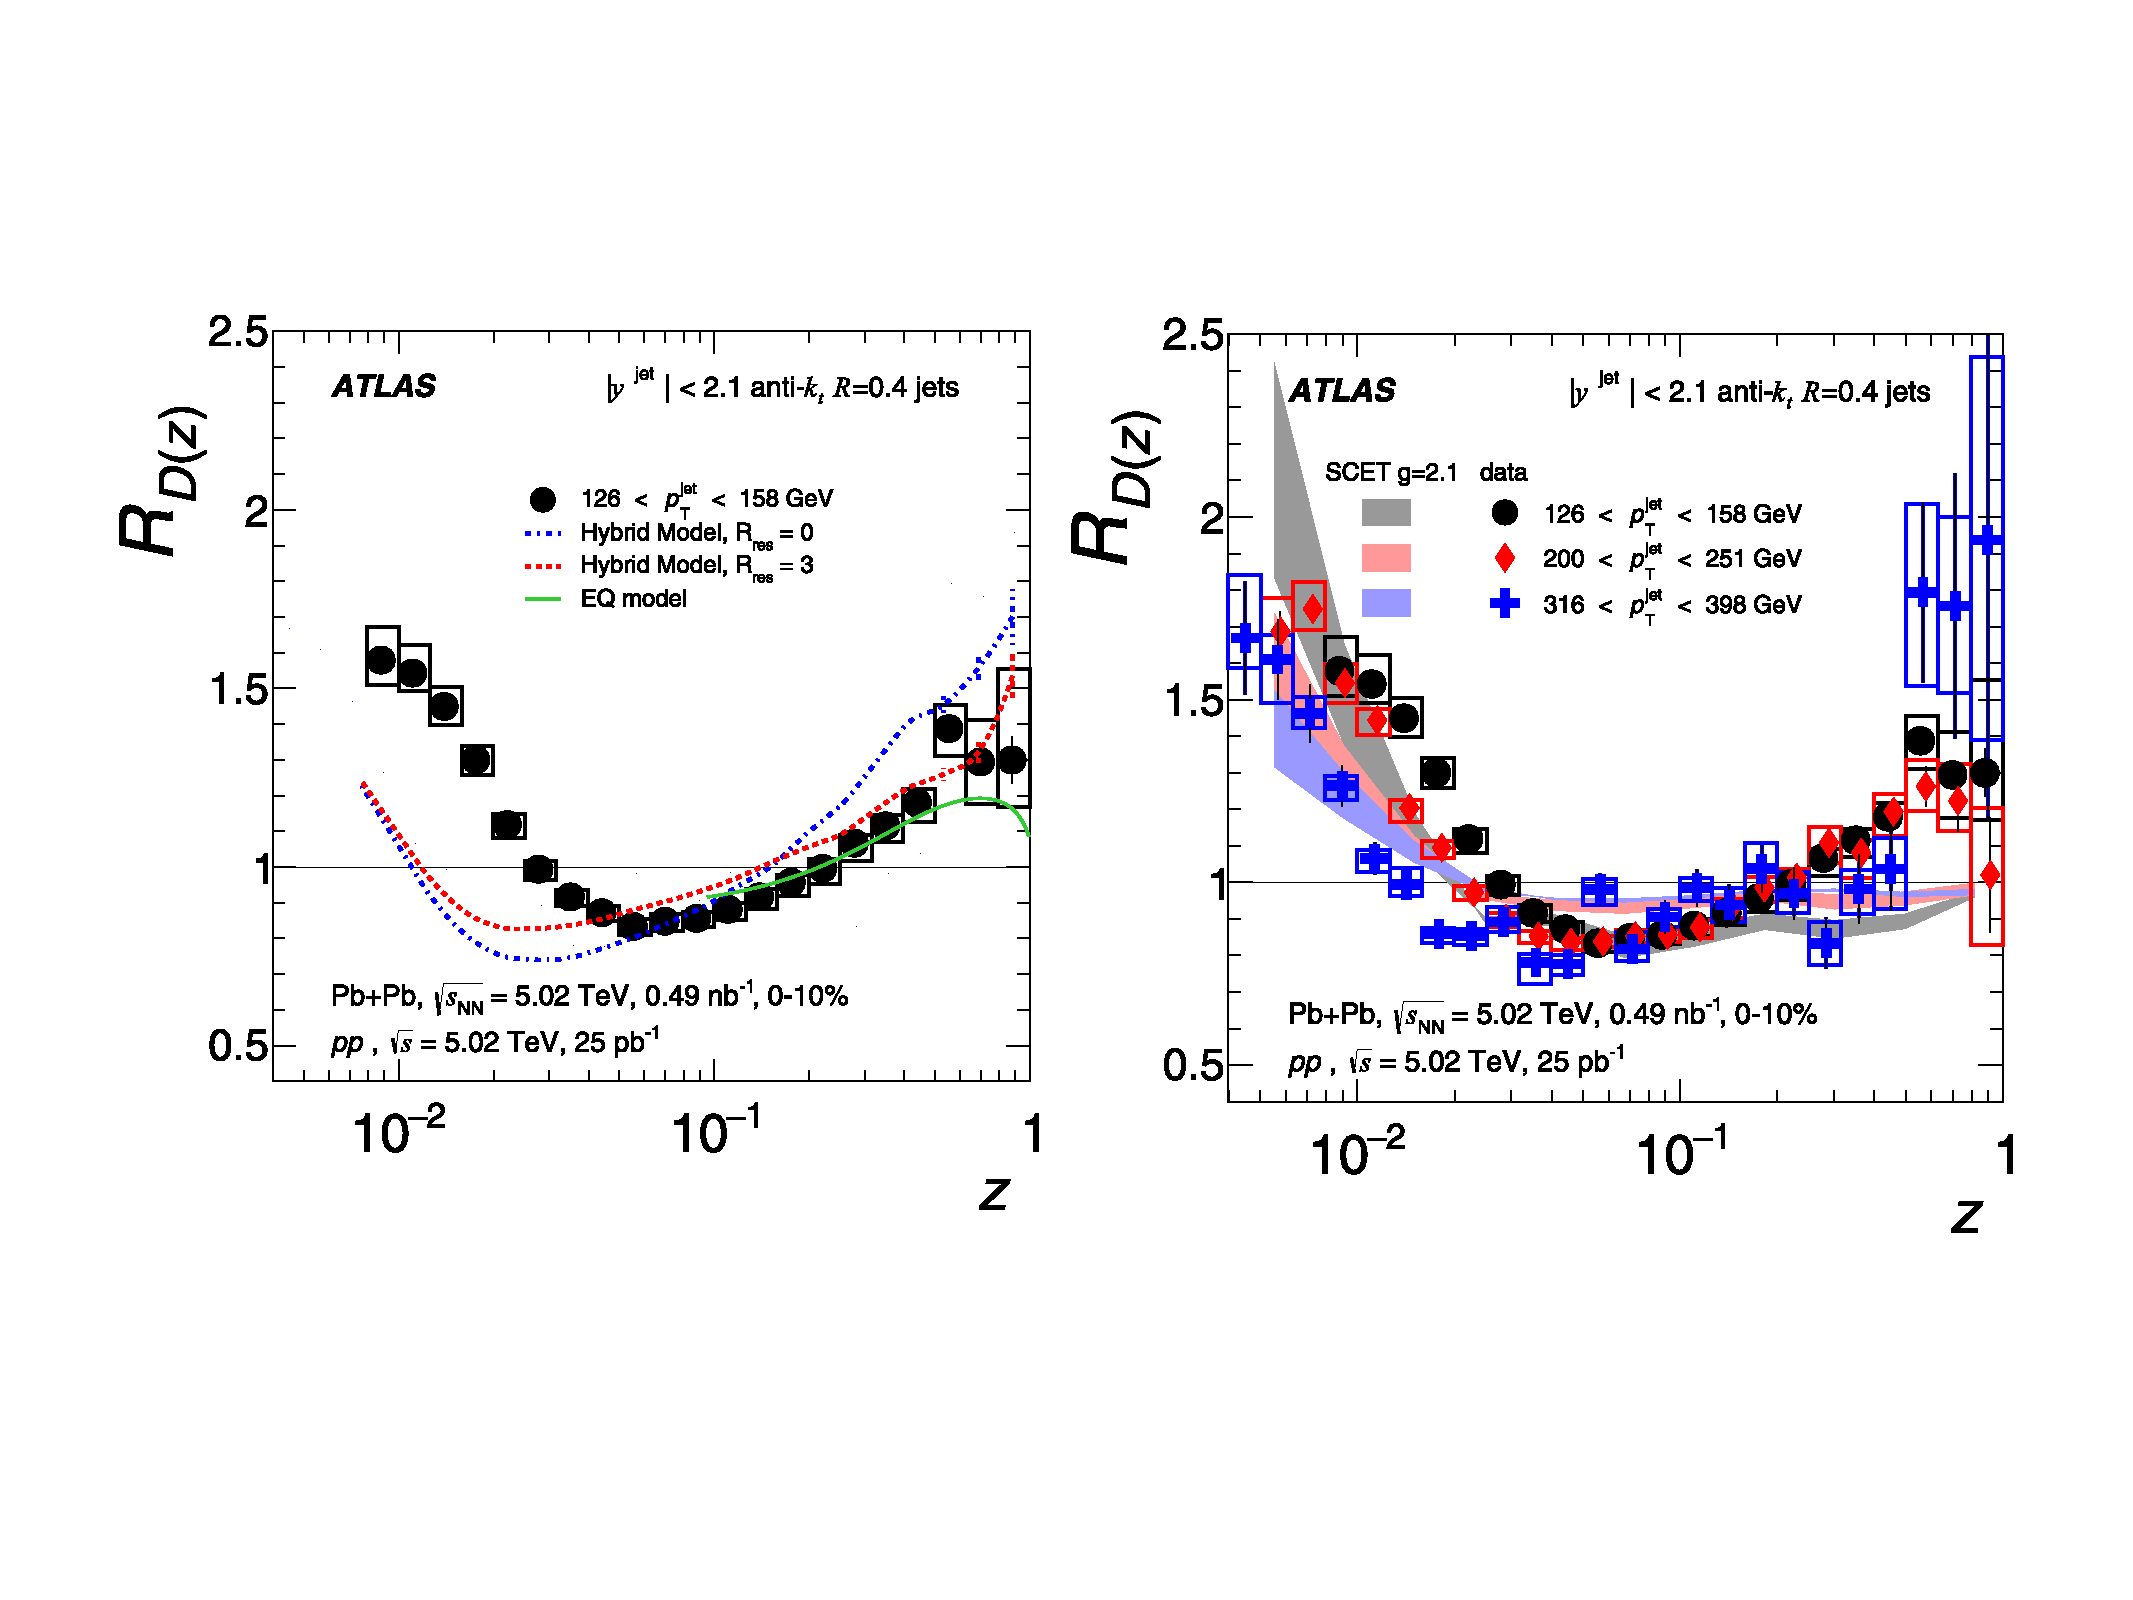
\includegraphics[width=0.75\textwidth]{figures/jetMeasurements/jetff_rdz_theory}
\caption{The \Rdz\ distributions compared to the EQ and Hybrid models (left) and SCET (right).
The error bars represent statistical uncertainties while the shaded boxes represent systematic uncertainties.
Figure taken from \cite{PhysRevC.98.024908}.}
\label{fig:jetff_rdz_theory}
\end{center}
\end{figure}



